\documentclass{article}

% if you need to pass options to natbib, use, e.g.:
\PassOptionsToPackage{numbers, compress}{natbib}
% before loading nips_2016
%
% to avoid loading the natbib package, add option nonatbib:
% \usepackage[nonatbib]{nips_2016}

% \usepackage{nips_2016}

% to compile a camera-ready version, add the [final] option, e.g.:
\usepackage[final]{nips_2016}

\usepackage[utf8]{inputenc} % allow utf-8 input
\usepackage[T1]{fontenc}    % use 8-bit T1 fonts
\usepackage{hyperref}       % hyperlinks
\usepackage{url}            % simple URL typesetting
\usepackage{booktabs}       % professional-quality tables
\usepackage{amsfonts}       % blackboard math symbols
\usepackage{nicefrac}       % compact symbols for 1/2, etc.
\usepackage{microtype}      % microtypography
\usepackage{subcaption}
\usepackage{amsmath}

% Figures
\usepackage{graphicx}
\graphicspath{ {../images/} }

\title{Artistic Style Transfer for Music Data}

% The \author macro works with any number of authors. There are two
% commands used to separate the names and addresses of multiple
% authors: \And and \AND.
%
% Using \And between authors leaves it to LaTeX to determine where to
% break the lines. Using \AND forces a line break at that point. So,
% if LaTeX puts 3 of 4 authors names on the first line, and the last
% on the second line, try using \AND instead of \And before the third
% author name.

\author{
  Patrick~Coleman, David~Penco, Adam~Porisky \\
  Department of Computer Science\\
  University of British Columbia\\
  \texttt{\{padsterpat, dpenco1, adam.porisky\}@gmail.com} \\
}

\begin{document}
\bibliographystyle{plain}

\maketitle

\begin{abstract}
  Recent work in the area of deep learning demonstrates that for 2D image data, style and content can be learned independently using convolutional neural networks (CNNs). The neural representation of style and content for two different images can be combined to generate a new image with the content of one image shown in the style of the other. We hypothesize that this method can be applied to music data to achieve a similar effect. Standard visual representations such as spectrograms or mel-frequency cepstrum coefficients (MFCCs) represent sound data in two dimensions, just like images. We directly apply the neural style transfer algorithm to these sound images and transform the result back into audio to generate new sounds with the content of one song and the genre or style of another. In addition, different loss functions that exploit the inherent structure of sound data are explored in an attempt to improve performance. 
\end{abstract}

\section{Introduction}

The application of machine learning principles to artistic or musical data is a unique and ongoing challenge. Machine learning is a powerful tool when it comes to classification of music and other forms of artistic media. Specifically, it is well-documented that deep learning and convolutional neural networks (CNN) allow for feature identification and subsequent categorization of audio content \citep{feng2014, Li2010}. However, a more difficult challenge exists in generating new, compelling artistic content. Projects such as DeepDream, artistic style transfer \citep{Gatys2015}, and NSynth by Magenta \citep{nsynth2017} are all examples of recent endeavours in this field.

Recent work done by Gatys et al. \citep{Gatys2015} demonstrates that for 2D image data, style and content can be learned independently using CNNs. The activations from two different images, one image for style and one image for content, can be used to reconstruct a new output image. This new image preserves the global arrangement and layout of the content image, but with the appearance of the style input image. We propose that this method can also be applied to music data to achieve a similar effect. We use standard visual representations such as spectrograms or mel-frequency cepstrum coefficients (MFCCs) to represent sound data in a format that is compatible with the neural style transfer algorithm. We then apply the neural style transfer algorithm to these sound images. Transforming the output back into audio generates a new sound file with the content of one song and the genre or style of another.

The loss function implemented by Gatys et al. is a combination of squared-error loss between the feature representations of the output image and the content image, and mean-squared distance between the values of the Gram matrices of the output image and style image \citep{Gatys2015}. To take advantage of the inherent structure that exists within spectrograms and MFCCs, we adjusted the loss functions for the CNNs used to train on the style and content images. We implemented a new loss function based on autocorrelations between horizontal and vertical pixels in an attempt to represent timing and harmonic patterns that exist in the audio data.

The main goal of our paper is to explore the feasibility of performing style transfer on audio data. In section 3 we describe a method for converting audio data into a form that is compatible with the existing neural style transfer algorithm. We also propose a new loss function capable of yielding better output spectrograms. In section 4 we compare the performance of the style transfer on audio data for different preprocessing steps and loss functions. In section 5 we discuss possible directions of future research.


\section{Related Work}

Our work builds upon the neural style transfer implemented by Gatys et al. The authors reconstructed photographs in the style of various well-known pieces of art \citep{Gatys2015}. They discovered that representations of the style and content of an image can be learned separately using unique loss functions. It is then possible to reconstruct a new image by performing gradient descent jointly using both the style and content loss functions. This results in an output image preserving the arrangement of one image, but with the texture and style of another. The two components are built into the loss function as distinct terms, allowing emphasis of style and content to be varied independently. These parameters are tuned by choosing the most visually appealing result. The applications investigated by the authors are limited to visual forms of media like paintings and photographs. We expand on their framework by modifying it and applying it to audio genre transfer tasks.

Representing sound data in a way that is usable by the neural style transfer algorithm is a key component in our work. As such, we investigated different features that could be used. Tzanetakis et al. propose sets of features to represent texture, rhythmic structure, and instrumentation for the purpose of genre classification \citep{Tzanetakis2001}. Audio data is divided into analysis windows from which features are caluclated, including centroid, rolloff, flux, zero-crossings, and energy. Other features included the mel-frequency cepstral coefficients (MFCCs) and autocorrelations of processed signals. MFCCs have proven to be especially useful in speech recognition tasks. Using these feature sets, each genre is modelled as a multivariate Gaussian and new audio is classified using standard Gaussian classification. Though our ultimate goal is not genre classification, selecting meaningful features that represent the audio in a way that is compatible with the neural style transfer algorithm is an important step.

The work done by Choi et al. also focusses on genre classification, but provides valuable insight into sound representation as well \citep{Choi2016}. The authors converted their audio clips into log-amplitude mel-spectrograms, stating that doing so outperforms standard MFCCs and linear-amplitude mel-spectrograms for genre classification tasks. They compared the performance of convolutional recurrent neural networks (CRNN) with three CNNs of varying structure in both memory-controlled and computation-controlled experiments. According to their results, CRNNs outperform CNNs with 2D convolution kernels when limited to the same number of parameters. However, computation using the 2D convolution kernels is faster.

\section{Applying Neural Style Transfer for Audio Data}

\textbf{Dataset.} \hspace{0.25cm} The dataset used in this paper is the Marsyas GTZAN genre collection. It consists of 1000 audio tracks with a length of 30 seconds each. The tracks are separated into 10 genres, each genre having 100 tracks. All of the tracks are recorded in 22050Hz Mono 16-bit audio. The data was originally collected and used by Tzanetakis et al. for genre classification, but has since been made publicly available \citep{Tzanetakis2002}. We trimmed the audio to 10 second clips and applied a bandpass filter as part of a preprocessing step. We chose a length of 10 seconds because it reduces the size of the data for computation purposes, and is still long enough to possess enough characteristic features to be recognized for a particular genre.

\textbf{Network Architecture.} \hspace{0.25cm} We implemented the same machine learning framework as the neural style transfer. The network is based on the 19 layer VGG-Network, a convolutional neural network intended to be used on 2D image data \citep{Simonyan2014}. It is important to note that the weights used for the VGG-Network are pre-trained using the ImageNet database \citep{Russ2014}. Features are acquired from the 16 convolutional layers and 5 pooling layers, while ignoring the fully connected layers. More information on the configuration of the network can be seen in \citep{Gatys2015}.

\textbf{2D Audio Representation.} \hspace{0.25cm} Spectrograms and MFCCs are two methods by which audio data can be represented in two dimensions. A spectrogram is a plot of the intensity of the short-time Fourier transform (STFT). Sound data is first sectioned into overlapping windows. The Fourier transform is applied to each window and the results are output as a vertical line. This vertical line represents the intensity at different frequencies. The transform is applied to all of the windows, and the output vertical lines are arranged in order of time. This results in an intensity plot with the horizontal axis representing time, and the vertical axis representing frequency. MFCC plots are also short-term, spectral based features and can be interpreted as a spectrogram with additional processing. To obtain MFCC features, we take the logarithm of the amplitude from the spectrogram, map the results to the mel scale, and then perform a discrete cosine transform \citep{Logan2000}. The mel scale accounts for the difference between actual frequency and perceived pitch. Like the spectrogram, the resulting image plots frequency as a function of time. An example of the spectrogram and MFCCs for the same sound clip is shown in Figure 1.

\begin{figure}[h]
\begin{subfigure}{\textwidth}
  \centering
  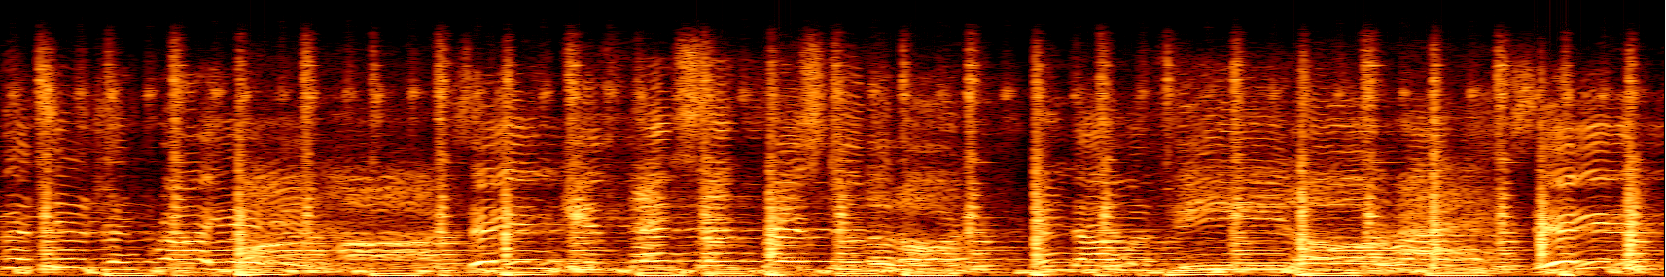
\includegraphics[width = \textwidth]{spec_example}
  \caption{}
\end{subfigure}
 \begin{subfigure}{\textwidth}
  \centering
  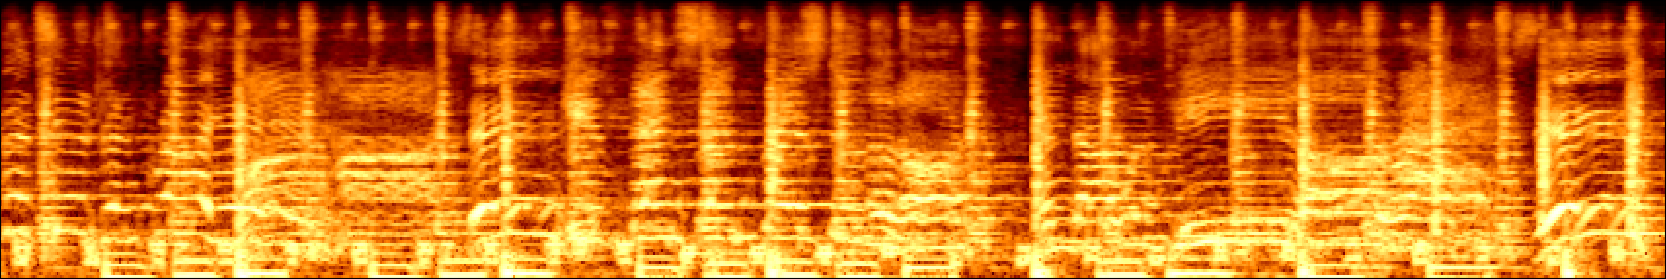
\includegraphics[width = \textwidth]{mel_example}
  \caption{}
\end{subfigure}
\caption{(a) Spectrogram transformation of audio clip. (b) MFCC transformation of audio clip.}
\end{figure}

\textbf{Loss Function.} \hspace{0.25cm} The original neural style transfer paper minimized two loss functions, one for content match and one for style match. For generated image features $F$, content features $P$, and style features $A$, these functions were defined as:
\begin{align*}
\mathcal{L}_{content}(\text{layer } l) &= \frac{1}{2} \sum_{i, j} (F_{i, j}^{l} - P_{i, j}^{l})^2 \\
\mathcal{L}_{style}(\text{layer } l) &= \sum_l \frac{1}{4N_l^2M_l^2}\sum_{i,j}(G_{i,j}^l(F) - G_{i,j}^l(A))^2
\end{align*}
where we denote the Gram matrix for layer $l$ by $G_{i,j}^l(X) = \sum_k X_{i,k}^l X_{j,k}^l$. 

In this paper, we introduce two new loss functions that capture properties more useful in the audio domain - specifically, beat and harmonic frequencies. In the context of a spectrogram, the beat pattern can be thought of as the correlation of the signal power with a delayed version of itself. The music should have a much stronger correlation when delayed the length of a beat, compared to a delay of a shorter length. This is captured by the row-wise autocorrelation for each frequency across time. Similarly, the power strength within a column of the spectrogram captures the harmonics present in the recording. By incorporating column autocorrelation as a loss function, the resulting audio should match the harmonic structure of the input file to which it is being compared.

Mathematically we can define these two properties by the row- and column-wise autocorrelations within the feature matrices. Given image features $F$ as above, we can define to more loss functions by matching its row- and column-wise autocorrelations to the style image:
\begin{align*}
\mathcal{L}_{row^\star}(\text{layer } l) &= \frac{1}{M_lN_l} (R^\star(F^l) - R^\star(A^l))^2 \\
R^\star(A^l)_{:,j} &= A_{i,:}^l \star A_{i,:}^l \text{ the row autocorrelation, i.e.} \\
R^\star(A^l)_{i,j} &= \sum_k a_{i,k}^la_{i,k-j}^l \\
\mathcal{L}_{column^\star}(\text{layer } l) &= \frac{1}{M_lN_l} (C^\star(F^l) - C^\star(A^l))^2 \\
C^\star(A^l)_{:,j} &= A_{:,j}^l \star A_{:,j}^l \text{ the column autocorrelation, i.e.} \\
C^\star(A^l)_{i,j} &= \sum_k a_{k,j}^la_{k-i,j}^l \\
\end{align*}

The final loss function is a weighted sum of all four components:
$$
\mathcal{L}_{total} = \alpha \mathcal{L}_{content} + \beta \mathcal{L}_{style} + w_{row} \mathcal{L}_{row^\star} + w_{col} \mathcal{L}_{column^\star}
$$
For this paper, we ran with weights $\alpha = 1\times10^{-3}, \beta = 2\times10^{5}, w_{col} = w_{row} = 1\times10^{-9}$. Additionally, while the content and style layers were the original ones taken from activations within the VGG network, the autocorrelation loss were defined over the input layer, to optimize calculation efficiency.

Note that autocorrelation of a vector is equivalent to convolution with its own reversal, which makes it easy to include within any system that runs convolutional neural networks.

\section{Experiments}

\subsection{Experimental Setup}

To test the algorithm we selected one content audio clip and one style audio clip from the Marsyas GTZAN genre collection database. We chose content and style from two distinct genres to exaggerate any differences. For the results shown in this paper, the content audio is from a song classified in the rock genre and the style audio is from a song classified in the reggae genre. Spectrograms for the two audio clips are shown in Figure 2.

\begin{figure}[!ht]
\begin{subfigure}{\textwidth}
  \centering
  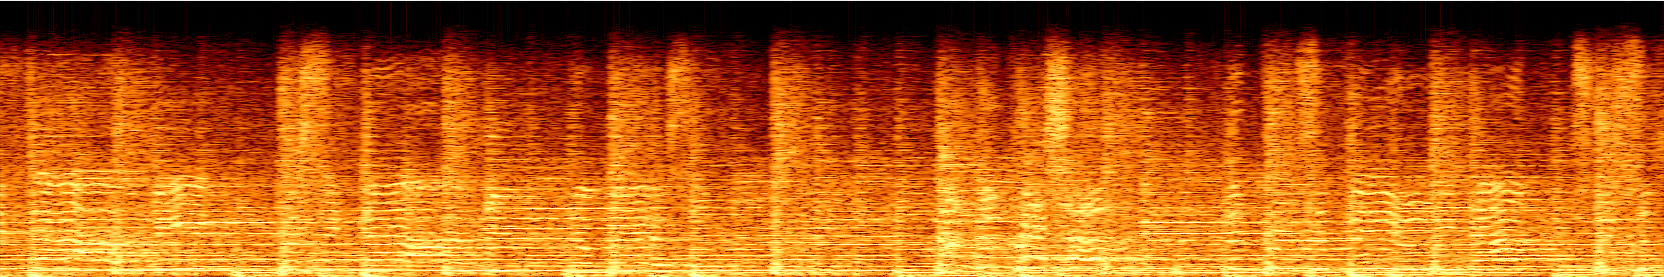
\includegraphics[width = \textwidth]{content_spec}
  \caption{}
\end{subfigure}
\begin{subfigure}{\textwidth}
  \centering
  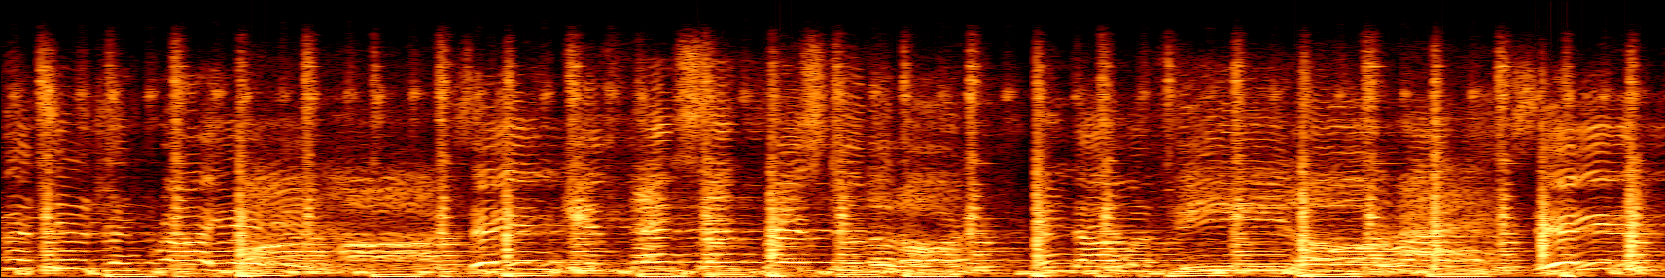
\includegraphics[width = \textwidth]{style_spec}
  \caption{}
\end{subfigure}
\caption{Spectrograms of the input audio files. (a) Rock genre content clip \#17. (b) Reggae genre style clip \#7.}
\end{figure}

Once our audio data is converted into a 2D form that is compatible with the neural style transfer code, the style transfer is applied. Gradient descent is performed on a white noise image with a goal of matching the feature responses as defined by our loss function. We implemented a different number of iterations for the two different formats that we used as inputs. For spectrograms gradient descent was performed for 25 iterations. For MFCCs 40 iterations were performed. This is because spectrograms have a higher resolution and require more time per iteration.

Code implementing the transfer (and all other stages of processing) was written in Python using the Lasagne and Theano libraries. It is available at \url{https://github.com/padster/AudioStyle}. Results were obtained running on an AWS GPU instance (at the time of writing: one p2.2xlarge, with a single NVIDIA K80 GPU), taking approximately 10 minutes to complete a transfer. 

\subsection{Results: Spectrograms}

As the results are generative and audio-based, there is no objective measure by which to grade the generated audio. Thus, the results were evaluated subjectively, as in the original transfer paper. Audio results can all be heard at \url{https://padster.github.io/AudioStyle/index.html}. Here we will primarily discuss the output spectrograms.

\begin{figure}[!h]
\begin{subfigure}{\textwidth}
  \centering
  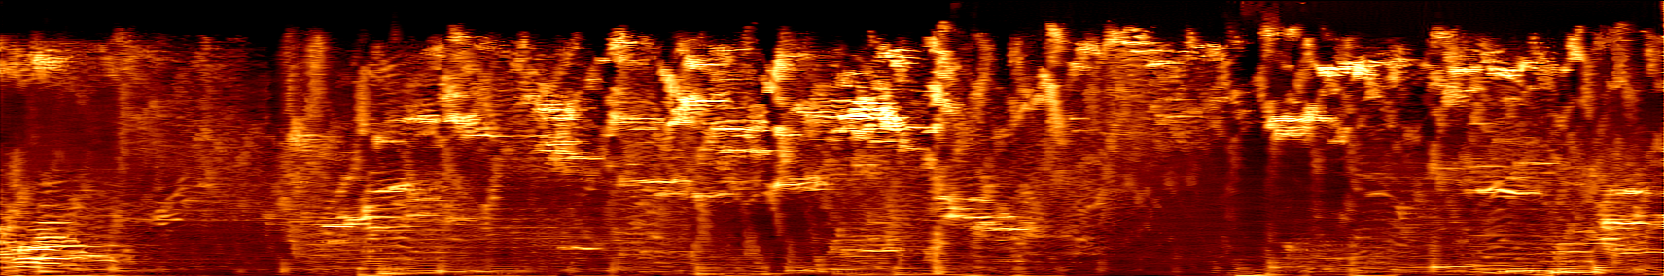
\includegraphics[width = \textwidth]{out1_spec}
  \caption{}
\end{subfigure}
\begin{subfigure}{\textwidth}
  \centering
  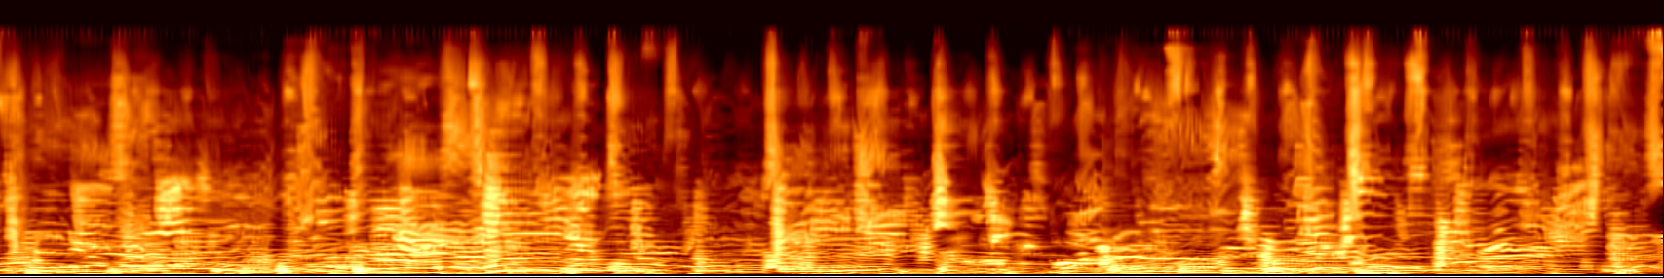
\includegraphics[width = \textwidth]{out2_spec}
  \caption{}
\end{subfigure}
\begin{subfigure}{\textwidth}
  \centering
  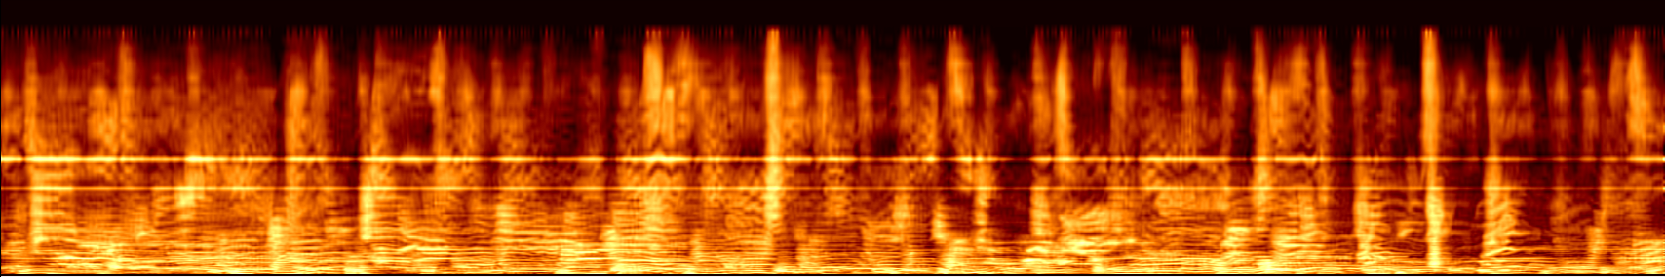
\includegraphics[width = \textwidth]{out3_spec}
  \caption{}
\end{subfigure}
\begin{subfigure}{\textwidth}
  \centering
  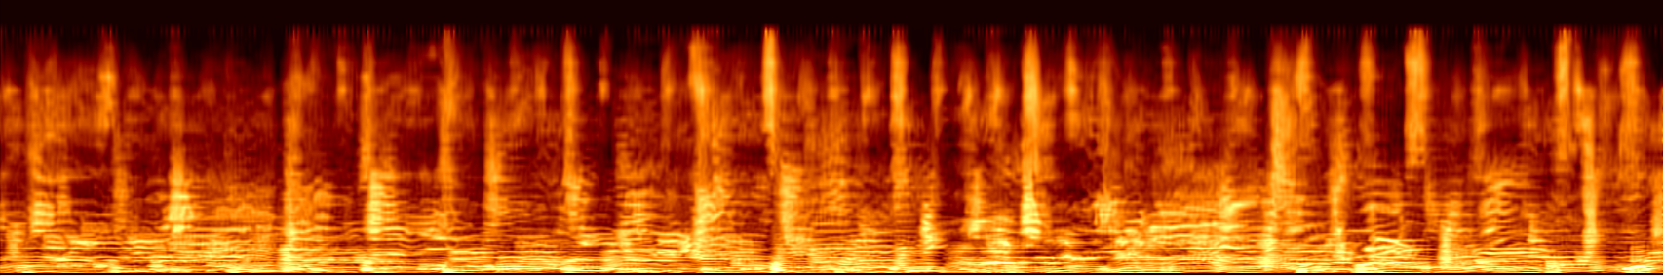
\includegraphics[width = \textwidth]{out4_spec}
  \caption{}
\end{subfigure}
\caption{Output spectrograms after style transfer using (a) original loss function (b) MFCC transform with original loss function (c) MFCC transform with row autocorrelation added to loss function (d) MFCC transform with row and column autocorrelation added to loss function.}
\end{figure}

Figure 3 shows the output spectrograms for four different style transfer experiments. Figure 3(a) is the result of applying the style transfer to the spectrogram of the input images. Figure 3(b) is the result of applying the style transfer to the MFCCs of the input images. Figure 3(c) also uses the MFCCs for the style transfer, but updates the loss function to include row autocorrelation. Figure 3(d) is the result of applying the style transfer to the MFCCs of the input images but implements both row and column autocorrelation in the loss function. In order to compare the results all of the images were converted back to spectrogram form.

As can be seen in Figure 3(a), the image transfer algorithm applied to spectrograms performed poorly. This is primarily due to the much larger image (1024 x 1712 after downsampling) reducing the number of optimization iterations. The result looks slightly like a spectrogram, but has none of the structure one would expect. This can be heard in the audio, which sounds the least musical of all four.

When applied the the MFCC version, the resulting spectrogram shown in Figure 3(b) appears much more like normal audio and does appear to visually mimic the style of the reggae spectrogram. However, due to the lack of positional constraints, there is no solid beat. This causes high and low frequencies to appear in isolation. The smaller image size of the MFCCs (96 x 854) allows for many more iterations of the style transfer algorithm to be performed in roughly the same amount of time.

After the row-based autocorrelation loss was included, the output appears to be more periodic along the horizontal axis. This is evident in Figure 3(c), where a distinct beat pattern can be seen. However, artifacts can also be seen in the result. Entire rows (i.e. frequencies) are erroneously optimized to higher values, which is possible under autocorrelation. When converted back to audio this results in a consistent, painful buzzing sound.

This is fixed by introducing the column autocorrelation loss. Figure 3(d) shows that using the updated loss function results in a spectrogram quite similar in style to that of the reggae song, while maintaining some of the same bright areas of the content. Although it still does not sound musical when converted back into an audio file, it does sound like the best representation of both style and content of the four.

\subsection{Results: Autocorrelations}

We can also verify that the autocorrelation losses are introducing the desired constraints on the generated spectrograms. For each row or column, we calculate the full autocorrelation, so it is twice the length, symmetric, and roughly linear. For presentation purposes, we first take the first-order pairwise difference to approximate the derivative, and average this out over all rows (or columns).

\begin{figure}[!h]
\begin{subfigure}{\textwidth}
  \centering
  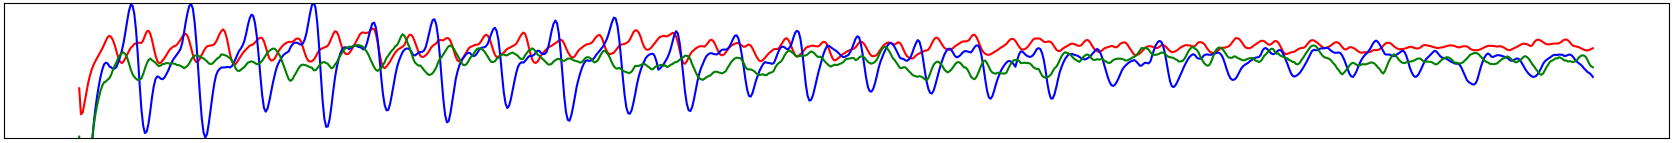
\includegraphics[width = \textwidth]{row_ac_mfcc_input}
  \caption{}
\end{subfigure}
\begin{subfigure}{\textwidth}
  \centering
  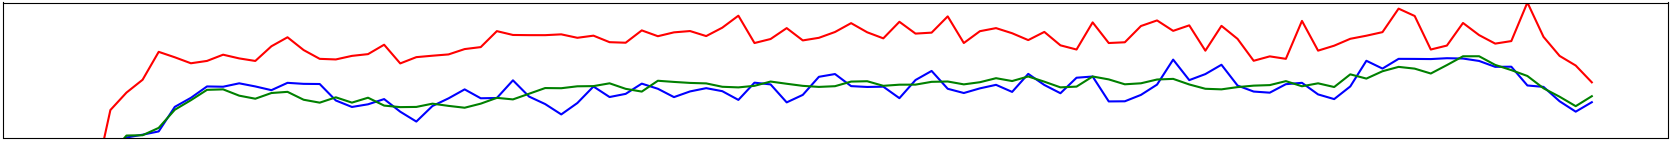
\includegraphics[width = \textwidth]{col_ac_mfcc_input}
  \caption{}
\end{subfigure}
\begin{subfigure}{\textwidth}
  \centering
  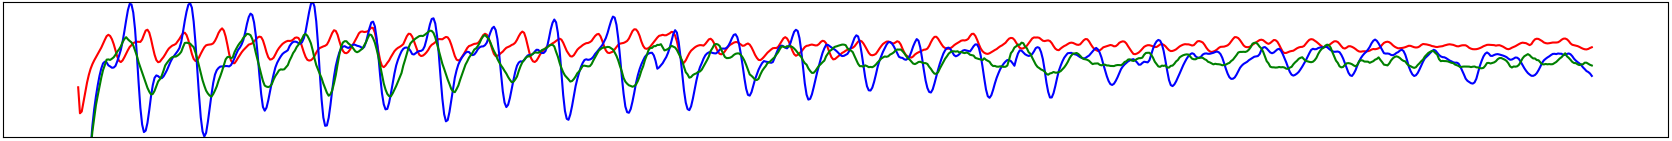
\includegraphics[width = \textwidth]{row_ac_input}
  \caption{}
\end{subfigure}
\begin{subfigure}{\textwidth}
  \centering
  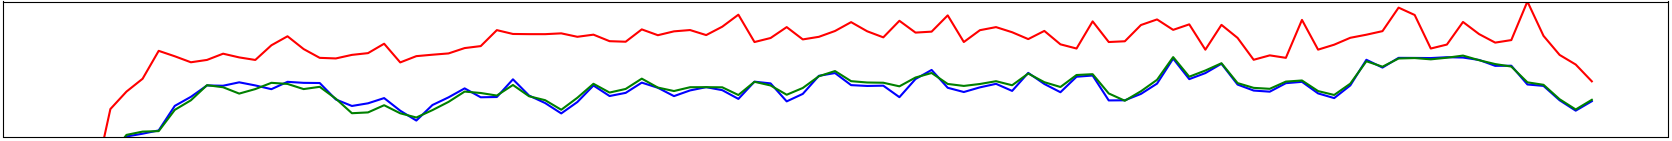
\includegraphics[width = \textwidth]{col_ac_input}
  \caption{}
\end{subfigure}
\caption{Autocorrelation plots. Red, blue, and green lines represent the content, style, and output images respectively. (a) Row autocorrelation for MFCC transformation. (b) Column autocorrelation for MFCC transformation. (c) Row autocorrelation for MFCC transformation with updated loss function. (d) Column autocorrelation for MFCC transformation with updated loss function.}
\end{figure}

Figures 4(a) and 4(c) show the average row autocorrelation derivatives, with and without the loss function applied. The beat of the rock content audio (red line) and reggae style audio (blue line) can clearly be seen in this graph. It is also possible to verify that, after the loss was added, the periodicity in the output audio (green line) is close to that of the style input, but with smaller amplitude. Though not shown here, similar periodicity can be seen in the activations for deeper layers of the network, even though the loss function was not included for these layers (calculation of the gradient for the deeper layers was too slow). Results for autocorrelations at multiple layers can be seen on the website with the audio outputs, mentioned previously.

Figures 4(b) and 4(d) show similar results for the average column autocorrelation derivates. These are much shorter and much flatter due to the nature of the audio structure. As would be expected, it can be seen in Figure 4(d) that the generated image matches the style image very closely once the column autocorrelation loss is included. Furthermore, we believe that using a different form of 2D representation could improve the information captured by the autocorrelation loss. Due to the nature of harmonic frequencies, a spectrogram with logarithmic frequency space (y-axis) such as constant-Q would be ideal.

\section{Discussion and Conclusion}

Our experiments suggest that representing audio data as MFCCs and implementing loss terms for row and column autocorrelation improves performance over simply using spectrograms. Not only does the resulting audio sound more like music with these changes, but it becomes less noisy and better captures the desired style content. However, further improvements are necessary. The output audio is still unpleasant to listen to even after using the MFCCs and the updated loss function.

In the resulting audio file, the content seems to be somewhat preserved, but with a considerable amount of noise. Only a few elements of the desired style have been successfully transferred, most notably the distinct percussive beats of the reggae composition. The end result sounds only somewhat like music, and loses all vocal components. Furthermore, the following processes and their respective inverses all contribute to audio quality losses: applying the FFT, applying the MFCC and applying the image style transfer. The resulting audio file has somewhat lower quality than would be desirable.

Another potential issue is that the VGG network we used was trained on general images from the ImageNet dataset rather than spectrograms, MFCCs or greyscale images, which would be more domain appropriate. One possible direction of future research would be to try training new weights using a more restricted image domain. We could also try representing the audio as a chromagram rather than a spectrogram, to capture the notes of the scale more explicitly. Other future research directions could include trying audio files with less complex composition, such as instrumentals. We could also try adjusting the weights, or reassigning the terms of the loss function. Currently, both autocorrelation terms of the loss function are applied to the style input. Applying both to the content input, or applying row autocorrelation and column autocorrelation separately could yield interesting results. For instance, it may be possible to match the beat of the content input using row autocorrelation, while transferring the harmonic structure from the style input using column autocorrelation loss.

Another broad challenge facing generative models such as our own is evaluation. It is easy to evaluate performance when categorizing art by style, or genre. Properly categorized test cases represent good performance, while misclassification is an example of poor performance. However, evaluation of performance becomes significantly more challenging when considering the output of generative models. Whether or not the result looks like art or sounds like music is typically subjective. Even subjectively this task becomes more difficult in the audio domain. Humans can quickly evaluate visual information, but limited to the rate of the recording when evaluating auditory information. As such, there exists a need to develop automatic, objective, and quantitative performance measures for generative tasks.

\bibliography{CPSC540_FinalReport}

\end{document}